% article example for classicthesis.sty
\documentclass[10pt,a4paper]{article} % KOMA-Script article scrartcl
\usepackage{lipsum}
\usepackage{url}
\usepackage[nochapters]{classicthesis} % nochapters
\usepackage{graphicx}
\graphicspath{ {../images/} }
\usepackage{multicol}

\begin{document}
	\pagestyle{plain}
	\title{\rmfamily\normalfont\spacedallcaps{Text Mining Twitter: Colombia 2018 Elections}}
	\author{\spacedlowsmallcaps{juan sebastián garcía rodriguez} \\ \spacedlowsmallcaps{travis dunlop}}
	\date{} % no date
	
	\maketitle
	
	\begin{abstract}
		\noindent Between May and June of 2018 the people of Colombia will vote for their next president.  As with any modern election, people are using Twitter, the social media platform, to support candidates they like, discredit the others, and debate who should win.  Twitter provides a massive open forum to create dialogue across the country.  Some groups take advantage of this by creating \textit{social bots}, which automatically post political tweets to in an attempt to sway votors \cite{swaine_2018}.  In our project, we use the text mining skills gained in this course to assess the influence of these bots.  We hope to answer two questions: what percentage of users tweeting about the election are bots and what is the sentiment of the tweets?
		
	\end{abstract}
	
	\section{Introduction}
		In order to answer these two questions we split the project into two sections:  bot detection and sentiment analysis.  For bot detection we leverage an existing algorithm and try both supervised and semi-supervised learning to extrapolate it's findings.  With sentiment analysis, we hand-labeled a portion of the tweets and use those to help classify the rest into positive, negative, or neutral. \\
		
	\section{Data Set}
	Since February we collected tweets that were related to the political situation and in specific about the Colombian elections for Senate and President. We collected 3.1 million of tweets from 3th of March to the 7th of May. We got information from 326,966 users and we have identified the following candidates: Gustavo Petro, Humberto de la Calle, Sergio Fajardo, Ivan Duque and German Vargas Lleras. Also, we collected tweets that were talking about politicians who are indirectly involved in the elections such as Alvaro Uribe and Claudia Lopez. We have this data set stored in a SQL data base and we used Python to process the data.
	\pagebreak
	
	\section{Bot Detection} 
		Dectecting social bots is a complicated phenomenon, because they usually aim to not be found.  This results in a game of cat-and-mouse - researchers attempting more sophisticated classification strategies, and bot-makers emulating increasingly human-like behavior.  One technique developed to identify bots is to use a \textit{honeypot}.  In this case, the honeypot is a set of researcher-created Twitter users who tweet mostly nonsense.  The users that interact with them are likely to be bots -- exploiting their desire to engage with many users.  Of course, some real users just happen to message or follow one of these bots.  In order to parse out which are the real, the researchers use unsupervised learning to cluster the data into groups.  They find that some of the clusters seem more human-like than others.  This particular strategy was developed and implemented by Lee et. all \cite{Lee2011SevenMW}. Once this group of bots are identified, features are extracted to compare them with other users.  The researchers use things like frequency of tweets, number of followers, time between posting, ratio of tweets to retweets, even the length of the username as features in the model.  Another group from the Indiana University Network Science Institute has made this model available as a API \cite{DavisVFFM16}.  Unfortunately, the API has limits on access and so, we label some users and then build a model to extrapolate our results to label other users. \\
		
		\noindent The features for the model is built by accessing Twitter's API for user data \cite{twitter}. We include as features:
		
			\begin{multicols}{3}
				\begin{itemize}
					\item account age
					\item tweets count
					\item friends count
					\item user description
					\item favorites count
					\item username length					
					\item location listed
					\item protected status
					\item default image
				\end{itemize}
			\end{multicols}
		
		To process the user description, we were heavily inspired by the paper by Hannes Mueller predicting conflicts from newspaper text \cite{mueller_rauh_2018}.  We first take the raw user description and create a bag-of-words model, converting each description into a vector where the entries are counts of each token.  With those vectors, we perform Latent Dirichlet Analysis utilizing the gensim package \cite{rehurek_lrec}.  We do this as method of feature engineering and dimension reduction.
		
		Since we only have labels for a portion of the users, we wanted to try a semi-supervised learning technique to leverage any underlying structure uncovered from the unlabeled data.  We used the Label Spreading method from the sklearn package \cite{scikit-learn}.  Unfortunately, it didn't work very well, managing an area-under-curve metric of 0.63.  So instead, we tried a Random Forest classifier that worked much better - area-under-curve of 0.83.  Below are the ROC curves for the two techniques.
		
		\begin{figure}[h!]
			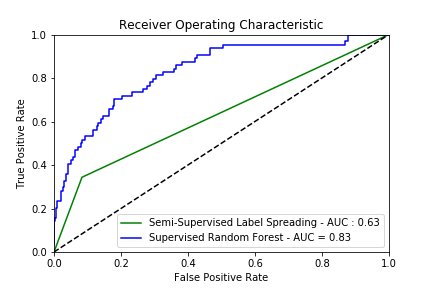
\includegraphics[width=0.8\linewidth]{roc_curve}
			\centering
		\end{figure}
	
	\pagebreak 
	
	In the end we had labels from 4,247 users and we had features from 8,721.  Of the whole dataset, we find that 3\% of them are bots.
		
	\section{Sentiment Analysis}
	In political times people tend to express more fiercely their feelings about the current situation in a country. This time Colombians has mixed feelings about what's next for the country since the peace deal is being implemented and Colombia is still living with crime and war. To approach such negative feelings we implemented topic modeling to extract weekly the hot topics in our data set and in parallel we train a model with a semi-supervised tecnique for learning the sentiment in those tweets. Respetively, we used a Latent Dirichlet Allocation(LDA) implementation from the package gensim and LabelSpreading from sklearn.
	
	\section{Conclusion}
	
	In the end, we have shown some evidence that
	
	% bib stuff
	\nocite{*}
	\addtocontents{toc}{\protect\vspace{\beforebibskip}}
	\addcontentsline{toc}{section}{\refname}
	\bibliographystyle{plain}
	\bibliography{project-report}
\end{document}